
\subsection{Comparison to existing approaches}

\begin{figure}[t]
	\centering
	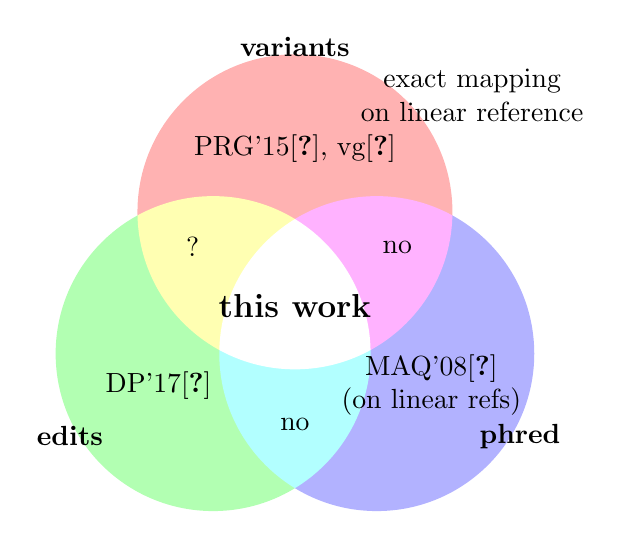
\begin{tikzpicture}
		\begin{scope}[blend group = lighten]
			\fill[red!30!white]   ( 90:1.2) circle (2);
			\fill[green!30!white] (210:1.2) circle (2);
			\fill[blue!30!white]  (330:1.2) circle (2);
		\end{scope}
		
		% labels
		\node at (90:3.3)    {\textbf{variants}};
		\node at (210:3.3)   {\textbf{edits}};
		\node at (330:3.3)   {\textbf{phred}};
		
		% 0 intersect (outside)
		\node [text width=3cm, align=center] at (50:3.5)    {exact mapping \\ on linear reference};
		
		% 1 intersect
		\node at (90:2)      {PRG'15\cite{dilthey2015improved}, vg\cite{VGtool}};
		\node at (210:2)     {DP'17\cite{rautiainen2017aligning}};
		\node [text width=3cm, align=center] at (330:2)     {MAQ'08\cite{maq2008mapping} \\ (on linear refs)};
		
		% 2 intersect
		\node at (150:1.5)   {?};   % between variants and edits
		\node at (270:1.5)   {no};  % between edits and phred
		\node at (30:1.5)    {no};  % between variants and phred
		
		% 3 intersect	
		\node [font=\large] {\textbf{this work}};
	\end{tikzpicture}
	\caption{Comparison of existing mapping approaches based on supported sources of uncertainty: different weighting of reference variants, edit distance minimization to reference, and query phred values} \label{fig:VennComparison}
\end{figure}

\fxwarning{Add columns to the comparison table: complexity, short/long read, single/pair-end, dataset, multiple reads (\eg extend from seed-and-extend, MSA)}
\fxwarning{Add rows to the comparison table: check with https://genome.cshlp.org/content/27/5/665.full.pdf\cite{paten2017genome}}
\begin{table*}
	\centering
	\begin{tabular}{lccccccccc}
		\toprule
		\bf{tool}  & \specialcell{\bf{reference}\\ \bf{graph}}  & \bf{variants}  & \bf{edits}  & \bf{phred}  & \specialcell{\bf{quality}\\ \bf{score}}  & \bf{probabilistic}  & \specialcell{\bf{no}\\ \bf{adhoc}}  & \bf{efficiency}  & \bf{evals} \\
		% tool+citation									& graph			& vars	& edits	& phred	&qual.score & prob	& not adhoc	& fast	& evals
		\midrule                                                                                                                    
		Smith-Waterman'81 \cite{smith1981comparison}	& linear		& \n	& \y	& \n	& \n	& \n			& \y	& \y	& ?		\\
		MAQ'08 \cite{maq2008mapping}					& linear		& \n	& (\n)	& \y	& \y	& \y (approx.)	& \y	& \y	& ?		\\
		Bowtie2'12 \cite{langmead2012fast}				& linear		& \n	& \y	& \n	& ?		& \n (ED)		& ?		& \y	& ?		\\ %SOAP'08, BWA'09, TopHat2'13
		Na'09 \cite{na2009alignment}					& linear		& \n	& \y	& \y	& ?		& \y ?			& ?		& ?		& exact alignment when changed DP scores	\\
		LAST'10 \cite{frith2010incorporating}			& linear		& \n	& \n	& \y	& \y	& \y ? 			& \n	& ?		& synth (subst+phred), real (on close specie)		\\
		BWA-MEM											& linear		& \n	& \n	& \n	& ?		& \n (MEM)		& ?		& ?		& ?		\\
%	GenomeMapper'09 \cite{schneeberger2009simultaneous} & ?				& ?		& ?		& ?		& ?		& \n (exact)	& ?		& ?		& ?		\\
		\midrule
		ERG'12 \cite{vijaya2012new}						& linear+variants?& ?	& ?		& ?		& ?		& ?				& ?		& ?		& RNA	\\
		BlastGraph'12 \cite{holley2012blastgraph}		& \y?			& \y	& (\y)	& \n	& \n    & \n			& \n	& \n	& \n	\\
		BWBBLE'13 \cite{huang2013short}					& many linear?	& \y	& ?		& ?		& ?		& ?				& ?		& ?		& ?		\\
		MuGI'14	\cite{danek2014indexes}					& many linear	& \y	& ?		& ?		& ?		& ?				& ?		& ?		& ?		\\
		\bf{GCSA'14} \cite{siren2014indexing}			& DAG*			& \y	& (\y) $\leq$ 3 & \n & \n & \n			& \y	& (\y) when ED is small	& mapping and variation on HG		\\
		HISAT2'15 \cite{kim2015hisat,siren2014indexing,langmead2012fast}
														& DAG*?			& \y	& ?		& \n	& ?		& ?				& ?		& \y	& \n?		\\
		PRG'15 \cite{dilthey2015improved}				& DAG			& \y	& (\n)	& \n	& \n	& ?				& \n	& \n	& only MHC genotypes	\\
		\bf{deBGA'16} \cite{liu2016debga}				& de Bruijn Graph& \y	& \n	& \n	& ?		& \n			& ?		& \y	& sim and real on HG		\\
		\bf{BGREAT'16} \cite{limasset2016read}			& DAG			& \y	& subst	& \n	& \n	& \n			& \n	& \y	& too simple \\
		Gramtools'16 \cite{maciuca2016natural}			& DAG			& \y	& \n	& \n	& \n	& \n			& \n	& \y	& \n	\\
		\bf{partis'16} \cite{ralph2016consistency}		& linear HMMs	& \y	& subst	& \n	& \n	& \y			& (\y)	& \n	& VDJ annotation	\\
		DP'17 \cite{rautiainen2017aligning}	(no tool)	& \y			& \y	& \y	& \n	& \n	& \n (ED)		& \y	& \n	& \n	\\
		Graphtyper'17 \cite{eggertsson2017graphtyper}	& DAG			& \y	& 1subst& \n	& \n 	& max.match		& ?		& \y	& only genotypes	\\
		VG'17 \cite{VGtool,paten2017genome,garrison2018variation}	& \y & \y	& \n	& \n	& ?	 	& \n (MEM)		& ?		& \y	& HG?	\\
		%FORGe'18 \cite{pritt2018forge}(preprint)		& DAG?			& \y	& ?		& ?		& ?		& ?				& ?		& ?		& ?		\\
		\bf{IGoR'18} \cite{marcou2018high}				& ?				& \y	& subst	& \n	& ?		& \n (ED)		& ?		& ?		& VDJ		\\
		\bf{BrownieAligner'18} \cite{Heydari2018}		& \y			& \y	& \y	& \n	& ?		& ?				& ?		& ?		& 		\\
		\bf{\tool}										& \y			& \y	& \y	& \y	& \y 	& \y			& \y 	& Dijkstra ($L N$ nodes, $L M$ edges)	& VDJ		\\
		\bottomrule
	\end{tabular}
	\caption{Comparison of existing mapping approaches (separate aligning steps not included).
		Edits are insertions, deletions and substitutions.
		MAQ accounts for edits after mapping.
		PRG accounts for edits after mapping and linearization.
		Only evaluated features are included. The DAG* can be extended to general graph.
	}
	\label{table:comparison}
\end{table*}

Multiple Genome Index(MuGI'14)

The Na'09 paper\cite{na2009alignment} aligns a read to another read.
They modify the edit penalties based on quality scores.
The evals are just counting how often the standard DP finds exactly the same alignment as the modified DP with the quality scores finds.

LAST'10\cite{frith2010incorporating} aligns a read to a genome allowing only for mismatches because of sequencing or wrong mapping.
The evals include both synthetic and real data.
In the simulated tests, they sample 36bp fragments with different levels of random substitutions (modeling the biological variation) and add noise from real phred values.
The real setting is xeno-mapping of reads from one specie to the genome of another closely related:
	firstly different sets of edit penalties are estimated, then three experiments are conducted: accounting for phreds, phreds+edits, phreds+edits+gaps.

The BlastGraph'12\cite{holley2012blastgraph} tool maps using seed hashing and aligns to the left and right of the seeds using DP minimizing edit distance.
It is evaluated on DBGs built using a 10K, 100K and 100K reads out of approx. 4M Illumina single-end 36nb reads (sra:DRR000096).
The edits compensate for technical noise but not for biological noise. The eval does not include bio variability.

Generalized compressed suffix array'14 (GCSA) is a BWT extention to graphs.
In order to support edits, full set of possible edits should be generated in the index.
It is built from a reference genome + known variation or by a multiple sequence alignment.
Indexes supporting ED of $\leq$ 0, 1, 2 and 3 are compared to RLCSA (Find and Locate) and BWBBLE (Find) on HG.
Evaluated on the Variation dataset'13\cite{}.
They find out that with increasing the allowed ED, mapping on the graph stops finding more or more unique mappings than on the linear reference (allowing for the same ED).

PRG'15\cite{dilthey2015improved} constructs a graph with edge probabilities by chopping reads to kmers. Then the whole reads are mapped to the graph and the two most probable haplotypes. This means that the reads are not mapped to an independent reference genome.

Gramtools'16\cite{maciuca2016natural} uses BWT to represent variations of the reference. Evaluated for speed not accuracy.

deBGA'16 \cite{liu2016debga} indexes a DBG and introduces a graph-based seed-and-extension algorithm.
``Generally, seed-and-extend aligners consist of two steps:
(i) seeding: the inference of putative read positions (PRPs) from the matches (hits) of tokens (seeds) between the read and reference genome;
and (ii) extension: alignment of the read to the region surrounding each PRP to determine the most likely read position(s)''
``One of the major bottlenecks faced by this approach is how to handle repetitive genomic regions, even in the context of a single genome,
for example, over 50\% of the human genome comprised repeats''
The evals measure the sensitivity and accuracy for read alignment against a single genome using simulated and real pair-end reads.
Compared to Bowtie2, BWA, BWA-MEM, STAR, SeqAlto and GEM.

ERG'16 \cite{vijaya2012new}.

BGREAT'16\cite{limasset2016read} maps single-end reads on DBGs using an exhaustive solution and a greedy speedup.
Evals consist of comparing mapping percentable on contigs vs the graph, calculating percentage of reads that map on branching paths.
The accuracy evals are only with sythetic reads with sequencing errors from HG being mapped on the same HB DBG.
Could compare only to BlastGraph but it was too unstable.
We subsume this method as the DBG can be converted to \tool.

Partis'16\cite{ralph2016consistency} precomputes the structure of a set of separate linear HMM for each VDJ recombination.
Then, based on the set of input sequences (\eg reads) it estimates allele usage probs, transition probs and emission probs and annotates each sequence by VDJ alleles.
Given a VDJ distribution and priors on gap size, naive sequences are simulated after which they are mutated (similar to BCR) into a set of sequences of a clonal family (using TreeSim).
Partis does inference by finding a path in the HMM that has maximum probability to generate a single or multiple sequences (multi-HMM).
The V, D and J allele correctness is compared to IMGT, IgBLAST, iHMMunealign and ighutil. Uses SW alignment.

Graphtyper'17\cite{eggertsson2017graphtyper} creates a DAG out of a reference and a set of variants.
Mapping is by hashing kmers (seed-and-extend) which are extracted from a read with 1bp overlap, then extending the seeds of overlapping kmers on the reference, then BFS through the graph structure of overlapping kmers (without any mistakes for now), then extracting kmers with 1 mistake from a read (and its reverse complement) that overlaps by 1bp. Evaluated are only genotype calls but not the alignments.

FORGe'18\cite{pritt2018forge} studies the drawbacks and trade-offs between accuracy and overhead when adding more reference genomes to the graph.
They suggest a method for scoring variants based on the effect on accuracy and the computational overhead and deciding which to add to the graph.
Compared to HISAT2, ERG,

IGoR'18\cite{marcou2018high} has 3 regimes: SW alignment, infer a model and evaluating sequence statistics. Compares to Partis and MiXCR using their own simulated data (instead of reusing). It does SW alignment.

BrownieAligner'18\cite{Heydari2018} works on de Bruijn graphs.
Claims alignment optimality but depends on initial heuristic seeding.
A Markov Model is built by aligning the reads on the graph, and then used for heuristically pruning the spurious paths. It captures more long-distance relationships than $k$.
Seems to use a cutoff of 2 indels for a banded DP.
Its scores (+1,-1,-3) are not general and what is most important, the matching score should be >0 (as commented in the code).
No phreds support. No probabilistic interpretation.
In the implementation, they perform DFS with a stack instead of priority queue (as shown in the paper).
They evaluate on simulated and on real reads from one genome: reads are simulated using ART tool\cite{huang2011art}, and the real reads true locations are assumed to be the ones found by bwa (no variant data).
B\&B speeds-up DFS between 1.1 times and 4-5 times.

In\cite{garrison2018variation} VG is evaluated by mapping simulated reads from a 150bp pair-end reads

As visualized on figure \ref{fig:VennComparison}, existing approaches regard some of the mentioned uncertainty sources but do not unify them in order to extract full advantage of the available data.
